% ============================================================
% APPENDIX A: TABLES (CSV files written by R/Q*.R in tables/)
% ============================================================
\section{Tables}\label{app:tables}

\subsection{Question 1}

\csvtable{q1a_variables}
  {Variables of the data set: name in R, original name, type and levels.}
  {tab:q1a-variables}

\csvtable{q1b_summary}
  {Summary statistics of the numerical variables (original data).}
  {tab:q1b-summary}

\csvtable{q1b_outliers}
  {Number of outliers ($1.5 \times \mathrm{IQR}$ rule) and of zero values of the numerical variables.}
  {tab:q1b-outliers}

\csvtable[\footnotesize]{q1b_removed}
  {Observations removed as impossible values: rule, removed values (\texttt{systolic}/\texttt{diastolic} for blood pressure) and number of rows.}
  {tab:q1b-removed}

\begin{table}[htbp]
  \centering
  \footnotesize
  \caption{Reference ranges of the health measures for adults. Sources: BMI \citep{who1995, who2000}, \texttt{body\_fat\_pct} \citep{ace_bodyfat}, \texttt{systolic} and \texttt{diastolic} \citep{nhs_hypotension, whelton2018} and \texttt{grip\_force} \citep{dodds2014}.}
  \label{tab:q1b-reference}
  \begin{tabular}{lll}
    \toprule
    Measure & Category & Range \\
    \midrule
    BMI (kg/m$^2$), from
      & Severe thinness       & $< 16$ \\
    \quad \texttt{height\_cm}, \texttt{weight\_kg}
      & Underweight           & $< 18.5$ \\
      & Normal weight         & 18.5--24.9 \\
      & Overweight            & 25--29.9 \\
      & Obesity               & $\geq 30$ \\
    \midrule
    \texttt{body\_fat\_pct} (\%),
      & Essential fat         & 2--5 / 10--13 \\
    \quad men / women
      & Athletes              & 6--13 / 14--20 \\
      & Fitness               & 14--17 / 21--24 \\
      & Average               & 18--24 / 25--31 \\
      & Obesity               & $\geq 25$ / $\geq 32$ \\
    \midrule
    \texttt{systolic} / \texttt{diastolic}
      & Low (hypotension)     & $< 90$ / $< 60$ \\
    \quad (mmHg)
      & Normal                & $< 120$ and $< 80$ \\
      & Elevated              & 120--129 and $< 80$ \\
      & Stage 1 hypertension  & 130--139 or 80--89 \\
      & Stage 2 hypertension  & $\geq 140$ or $\geq 90$ \\
      & Hypertensive crisis   & $> 180$ and/or $> 120$ \\
    \midrule
    \texttt{grip\_force} (kg),
      & Peak median (ages 26--42) & 51 / 31 \\
    \quad men / women & & \\
    \bottomrule
  \end{tabular}
\end{table}

\csvtable{q1b_shapiro}
  {Shapiro-Wilk p-value of the numerical variables (random sample of 5,000 observations of the cleaned data).}
  {tab:q1b-shapiro}
\csvtable{q1e_age_groups}
  {Frequency of each age group (\texttt{age\_cat}).}
  {tab:q1e-age-groups}

\csvtable{q1f_age_class}
  {Contingency table of age group and performance class.}
  {tab:q1f-age-class}

\csvtable{q1f_age_gender}
  {Contingency table of age group and gender.}
  {tab:q1f-age-gender}

\csvtable{q1f_chisq}
  {Chi-square tests of independence: statistic, degrees of freedom, p-value and smallest expected count.}
  {tab:q1f-chisq}

% ============================================================
% APPENDIX B: FIGURES (PNG files written by R/Q*.R in figures/)
% ============================================================
\clearpage
\section{Figures}\label{app:figures}

\subsection{Question 1}

\begin{figure}[htbp]
  \centering
  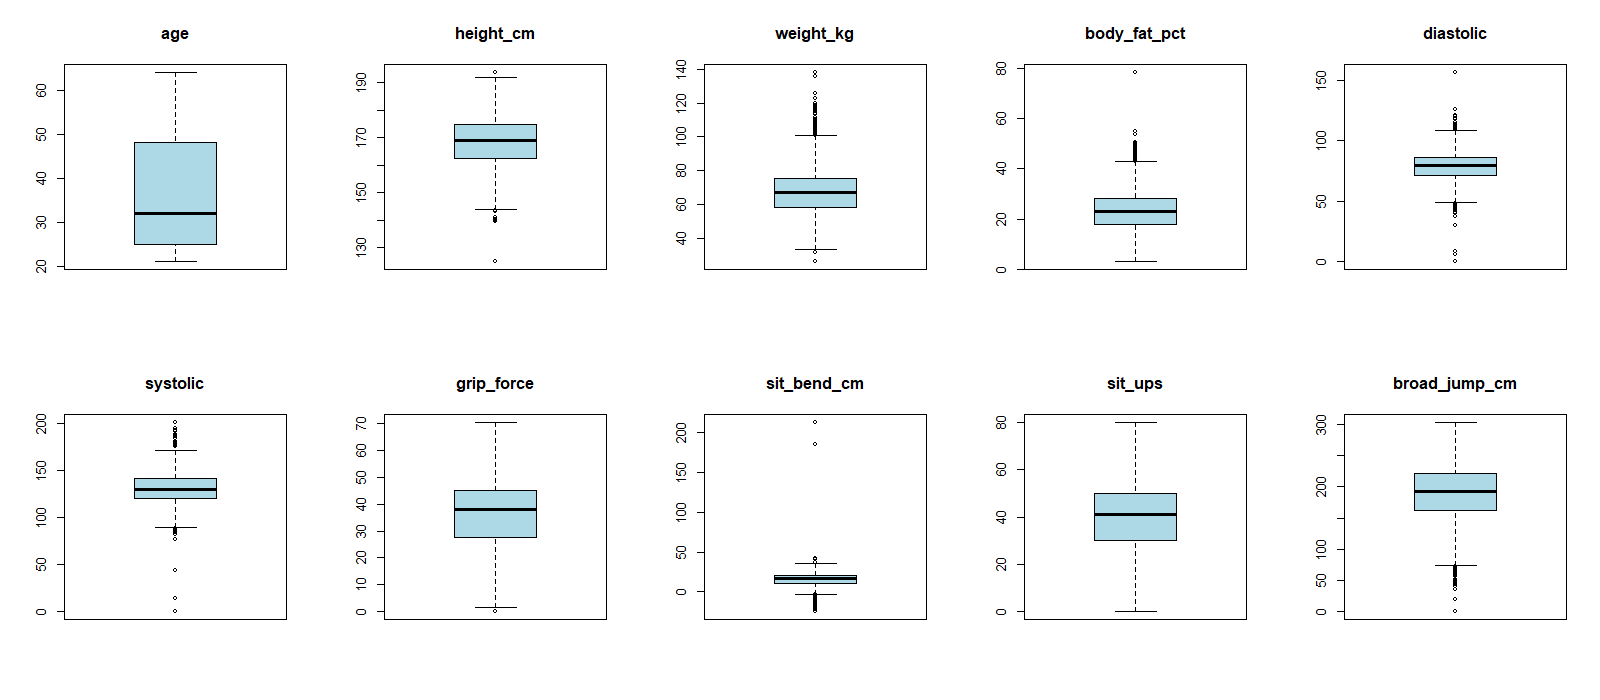
\includegraphics[width=\linewidth]{q1b_boxplots}
  \caption{Boxplots of the numerical variables (original data).}
  \label{fig:q1b-boxplots}
\end{figure}

\begin{figure}[htbp]
  \centering
  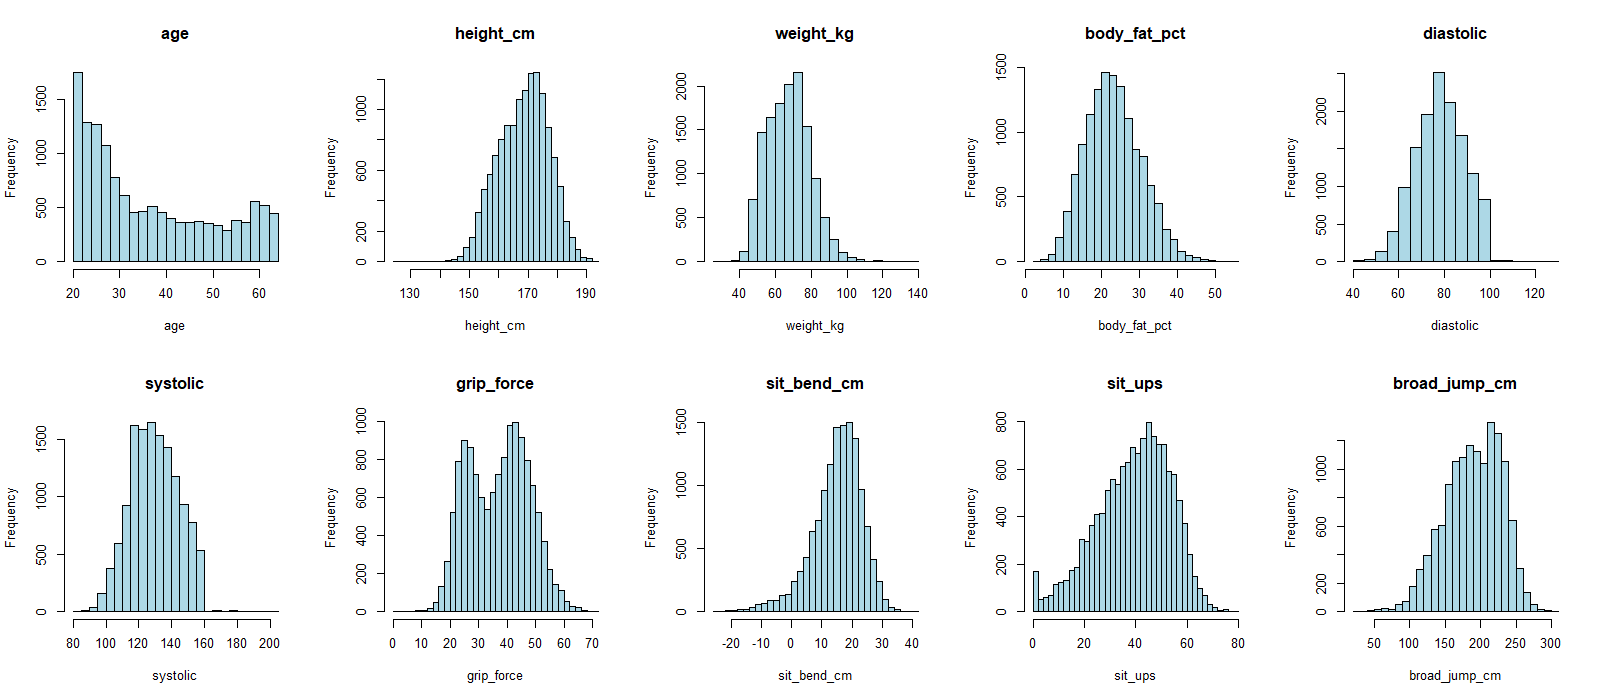
\includegraphics[width=\linewidth]{q1b_histograms}
  \caption{Histograms of the numerical variables (cleaned data).}
  \label{fig:q1b-histograms}
\end{figure}

\begin{figure}[htbp]
  \centering
  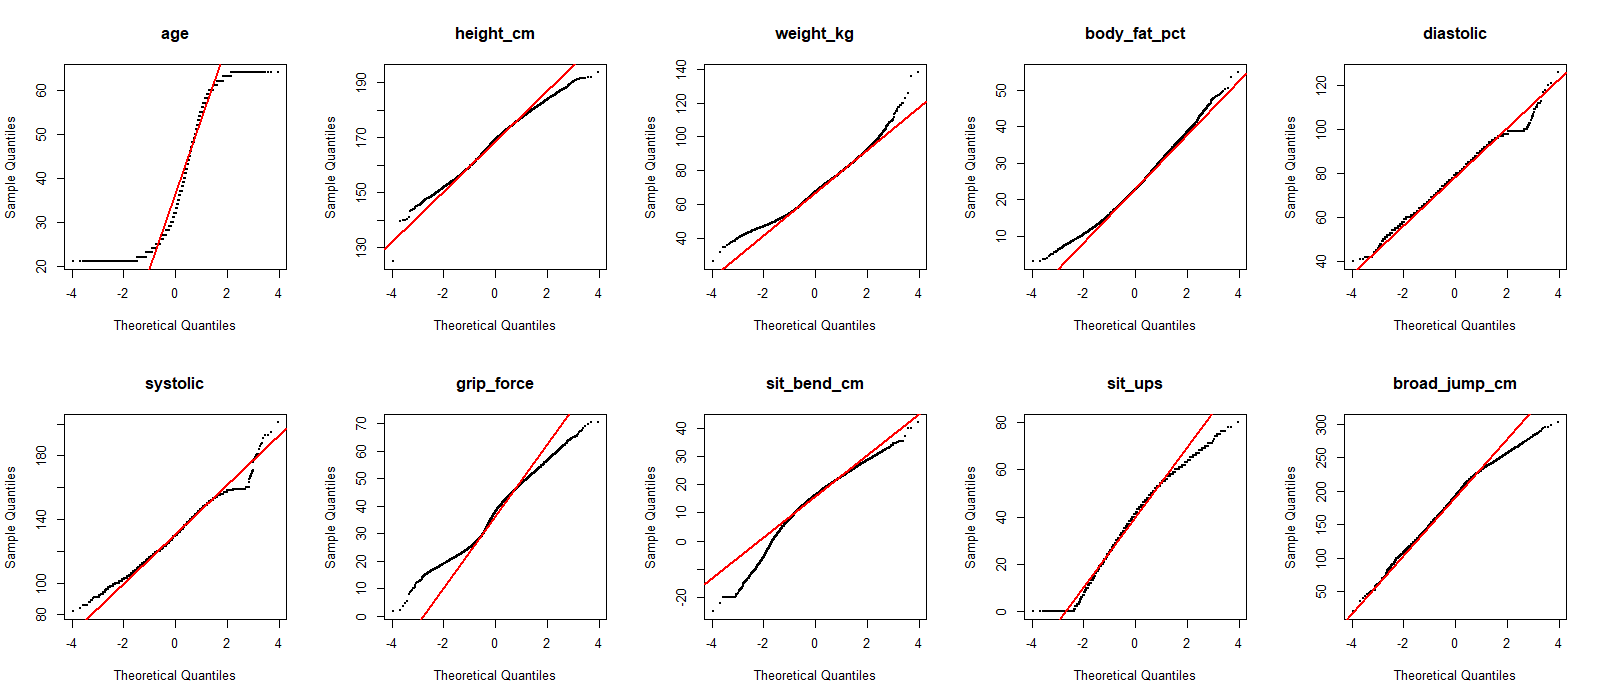
\includegraphics[width=\linewidth]{q1b_qqplots}
  \caption{Normal Q-Q plots of the numerical variables (cleaned data; red line: normal distribution).}
  \label{fig:q1b-qqplots}
\end{figure}

\begin{figure}[htbp]
  \centering
  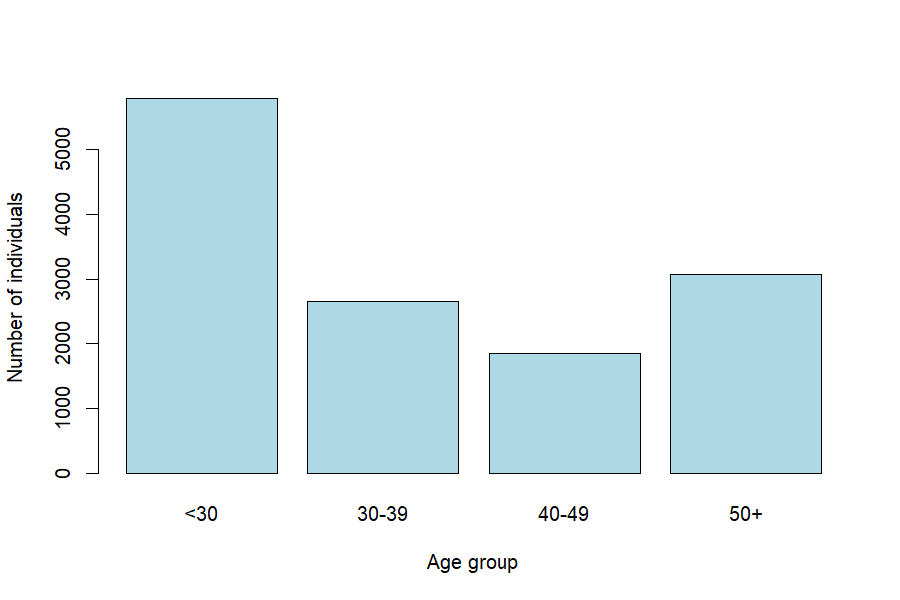
\includegraphics[width=0.6\linewidth]{q1e_age_groups}
  \caption{Number of individuals in each age group.}
  \label{fig:q1e-age-groups}
\end{figure}

\begin{figure}[htbp]
  \centering
  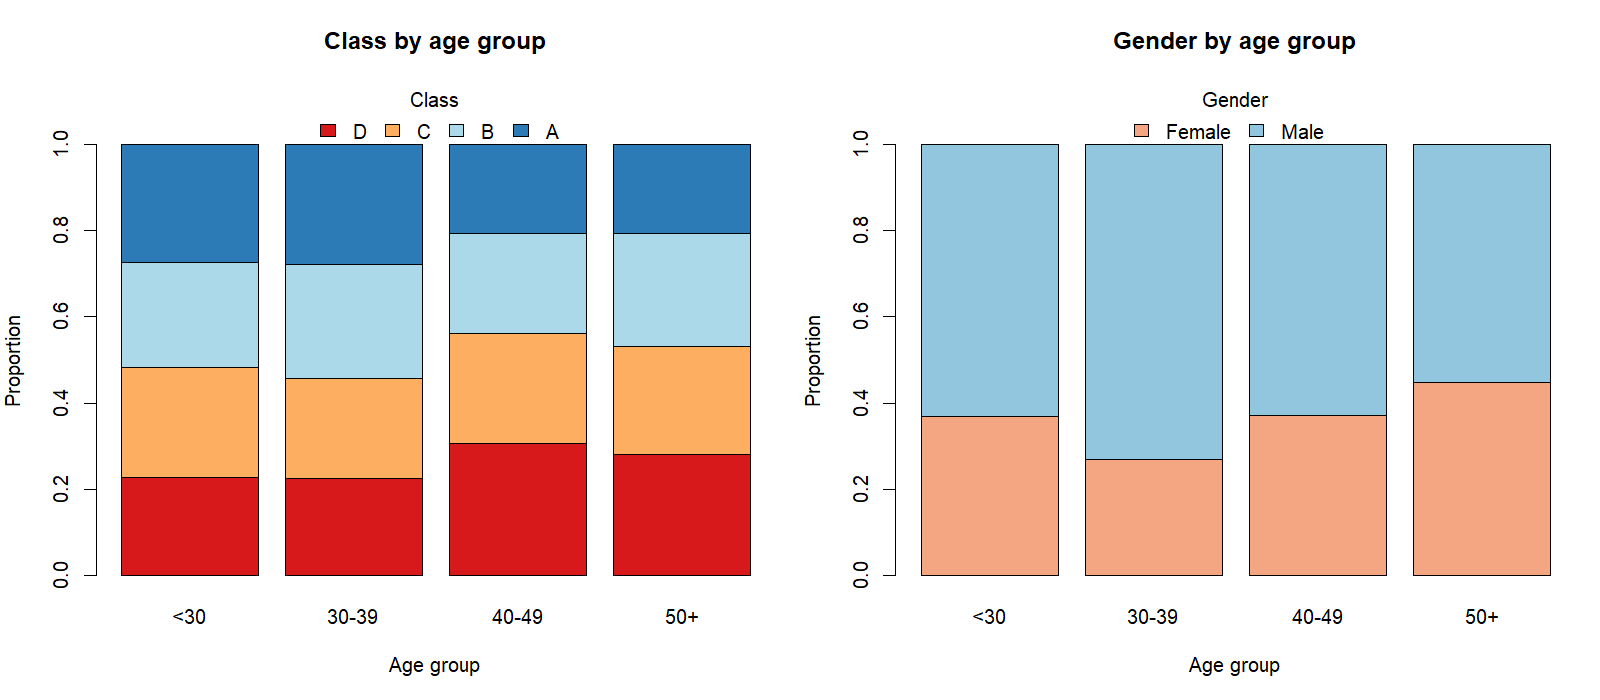
\includegraphics[width=\linewidth]{q1f_proportions}
  \caption{Proportion of each performance class (left) and gender (right) in each age group.}
  \label{fig:q1f-proportions}
\end{figure}

% ============================================================
% APPENDIX C: R CODE AND OUTPUTS
% ============================================================
\clearpage
\section{R Code and Outputs}\label{app:code}

The analysis is done in R, with one script per question in the \texttt{R/} folder of the project: \texttt{R/Q1.R}, \texttt{R/Q2.R} and \texttt{R/Q3.R}, with one section per part of the question.

Each script writes three kinds of output: the tables as CSV files (Appendix~\ref{app:tables}), the charts as PNG files (Appendix~\ref{app:figures}), and its full console output in a log, \texttt{R/logs/<script>.log}.

